{A right triangular cone with height of 10 and whose base is a right, isosceles triangle with side length 4.

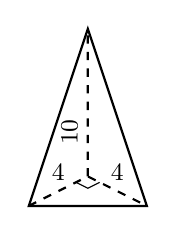
\begin{tikzpicture}[scale=.75]
\draw [thick](-1,0) -- (1,0) -- (0,3)--cycle;
\draw [thick,dashed] (-1,0) --  node [pos=.5,above] {\small 4} (0,.5) -- node [pos=.5,above] {\small 4} (1,0)
											(0,.5)-- node [pos=.3,above,rotate=90] {\small 10} (0,3);
\draw (-.2,.4) -- (0,.3) -- (.2,.4);
\end{tikzpicture}
}
{Orient the cone such that the tip is at the origin and the $x$-axis is perpendicular to the base. The cross--sections of this cone are right, isosceles triangles with side length $2x/5$; thus the cross--sectional areas are $A(x) = 2x^2/25$, giving a volume of $80/3$ units$^3$.
}
